\chapter{Optimization with uncertain graph weights}
\label{chap:unc_weights}

\section{Problem}
\label{sec:unc_w_problem}

In this scenario the only uncertain parameters are the graph weights.

Alongside the other operations, the learner will run a \textbf{graph estimation} algorithm to build an accurate representation of the graph at each time step.
Meanwhile, since the $\alpha$-functions are known, there is no need to estimate them and they can be applied directly in the optimization problem.

\section{Implementation}
\label{sec:unc_w_impl}

\subsection{Initial solution}

In the first interpretation of this assignment we set out to exploit graph influencing techniques in order to tackle this problem, however, in the long run the results were suboptimal and we decided to opt for a different approach.

Nonetheless, the graph influence related functions still exist in the codebase for posterity reasons, those are: \texttt{get\_influence\_per\_product}, \texttt{make\_influence\_graph} and \texttt{get\_influence\_of\_seed}.
The rationale for our graph influencing approach was based on determining how much each product was valuable to invest budget in by following activation patterns on the estimation of our graph, which contained our approximate weights.

In the end we opted for a more experimental approach that better exploited all of the information at our disposal in this particular step: by simulating the hypotethic behavior of a fixed set of people walking the graph, following our estimated weights and observing which products resulted in more return; we were able to produce meaningful budget assigments and tune the estimated graph weights over time following the behavior observed on real interactions.

\subsection{Prediction}

Since there is no need to estimate the $\alpha$-functions, the best allocation is calculated using the \texttt{find\_optimal\_superarm} function used to obtain the best estimation when the $\alpha$-functions are known.
The only difference is that a custom graph needs to be specified since we don't have access to the real graph weights.

\subsection{Graph estimation}

The learner contains a graph representation that is updated at each time step; the graph representation is not updated directly but through a function called \texttt{graph\_estimate}, which collects samples from various beta distributions for each graph weight, deleting \textit{self-loops} and non-existent edges.

The parameters of the beta distributions ($\alpha$ and $\beta$) are defined for each edge of the graph and represent the effective quantities that are updated whenever the function \texttt{learn} is called on the learner.

Whenever we want to make the graphless learner learn by calling its dedicated function, the learner analyzes all of the interactions given as a parameter and looks at the path that the users traversed by comparing it with the current graph representation.
If a certain edge is taken or not by a given user, the $\alpha$ and $\beta$ parameters are updated accordingly.
When \texttt{predict} is called again, the graph representation is then generated from scratch by drawing samples from the beta distributions with the updated parameters.

\subsection{Relevant code}

Implementation of the \texttt{predict} function:

\begin{lstlisting}[style=Python]
def predict(
	self, data: MaskedEnvironmentData
) -> Tuple[np.ndarray, Optional[List[List[Feature]]]]:
	budget_steps = np.linspace(0, data.total_budget, self.n_budget_steps)

	# Sample current estimation of graph
	graph = self.graph_estimation()

	best_allocation = find_optimal_superarm(data, budget_steps, custom_graph=graph)

	return budget_steps[best_allocation], None\end{lstlisting}

Implementation of the \texttt{learn} function:

\begin{lstlisting}[style=Python]
def learn(
	self, interactions: List[Interaction], reward: float, prediction: np.ndarray
):
	for interaction in interactions:
		remaining_edges = [
			(product, next_)
			for product, nexts in enumerate(self.next_products)
			for next_ in nexts
			# Only add edge to remaining if we visited the page, otherwise
			# we got no information about those edges
			if interaction.items_bought[product] > 0
		]
		for edge in interaction.edges:
			s, t = edge
			self.alpha_param[s, t] += 1
			remaining_edges.remove(edge)

		for edge in remaining_edges:
			s, t = edge
			self.beta_param[s, t] += 1
\end{lstlisting}

\section{Results}
\label{sec:unc_w_res}

\subsection{Single run reward and regret}

\begin{center}
	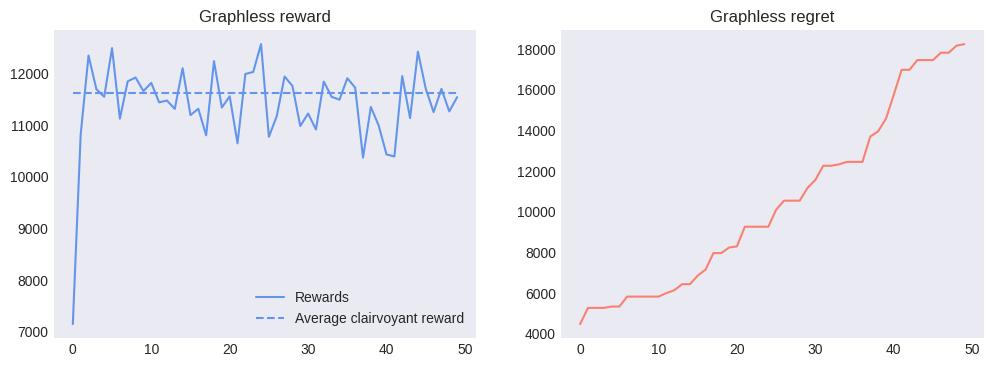
\includegraphics[scale=0.5]{img/Graphs/graphless/image1.png}
\end{center}

\subsection{Average reward and regret}

\begin{center}
	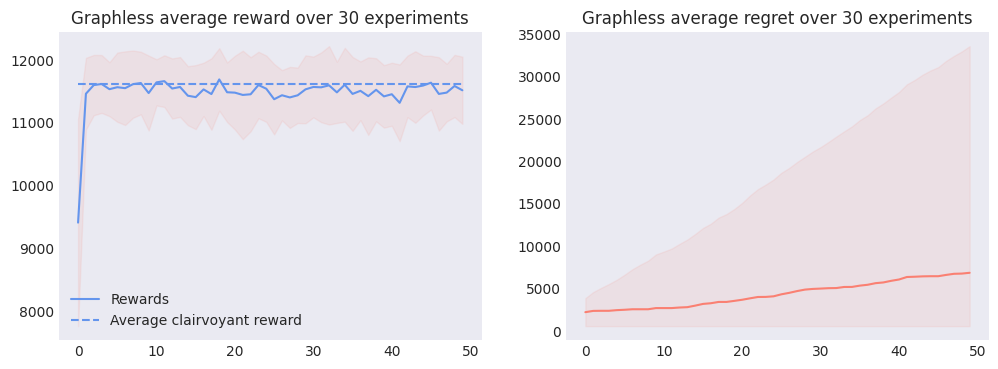
\includegraphics[scale=0.5]{img/Graphs/graphless/image2.png}
\end{center}

\subsection{Conclusions}

We can observe that the regret is exceptionally low w.r.t the previous learners, this is most likely due to the fact that the graphless learner has access to most of the important information from the environment and is able to give accurate estimations from the start.
However, some variance is always present due to the \textit{imperfect graph estimation} and \textit{environment non-determinism}.

Average results over 30 runs at time horizon $T = 50$:

\begin{table}[h]
	\center
	\begin{tabular}{|c|cc|c|}
	\hline \hline
		\cellcolor{blue!25} & Reward 	& Regret	& Deviation \\
	\cline{2-4}
		\cellcolor{blue!25} & $\mu$		& $\mu$		& $\sigma$	\\
	\hline \hline
		Graphless			& 11515.87 	& 6845.87	& 534.97 	\\
	\hline \hline
	\end{tabular}
\end{table}
